\documentclass[main.tex]{subfiles}
\begin{document}
\section{sorting}

There are many sorting algorithms, seriously, a lot, we saw 3 (or 4?) in class. For each algorithm I will discuss its best and worse execution case and why is so slow (or fast).

\subsection{Bubble sort}

The most basic of all the sorting algorithms, basically we go through every element and compare with its next element, if the next element is smaller than the current element we swap both:

\begin{figure}[htp]
    \centering
        \begin{subfigure}[b]{\textwidth}
            \centering
          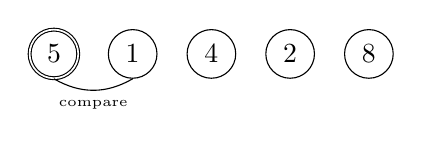
\begin{tikzpicture}
            \path (0,0) node[circle,double,draw] (A) {5};
            \path node[circle,draw,right of=A] (B) {1};
            \path node[circle,draw,right of=B] (C) {4};
            \path node[circle,draw,right of=C] (D) {2};
            \path node[circle,draw,right of=D] (E) {8};
        
            \begin{scope}[every node/.append style={midway}]
              \draw[bend right] (A.south) edge node[below]{\tiny compare} (B.south);
            \end{scope}
          \end{tikzpicture}
        \end{subfigure}
        \begin{subfigure}[b]{\textwidth}
            \centering
              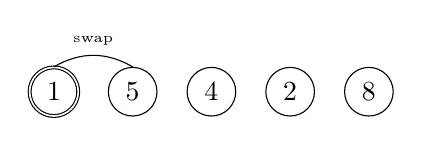
\begin{tikzpicture}
                \path (0,0) node[circle,double,draw] (A) {1};
                \path node[circle,draw,right of=A] (B) {5};
                \path node[circle,draw,right of=B] (C) {4};
                \path node[circle,draw,right of=C] (D) {2};
                \path node[circle,draw,right of=D] (E) {8};
            
                \begin{scope}[every node/.append style={midway}]
                  \draw[bend left] (A.north) edge node[above]{\tiny swap} (B.north);
                \end{scope}
              \end{tikzpicture}
        \end{subfigure}

        \rulesep

        \begin{subfigure}[b]{\textwidth}
            \centering
              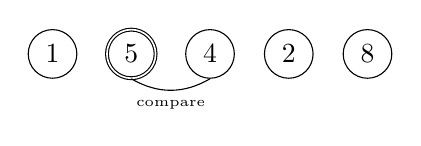
\begin{tikzpicture}
                \path (0,0) node[circle,draw] (A) {1};
                \path node[circle,draw,double,right of=A] (B) {5};
                \path node[circle,draw,right of=B] (C) {4};
                \path node[circle,draw,right of=C] (D) {2};
                \path node[circle,draw,right of=D] (E) {8};
            
                \begin{scope}[every node/.append style={midway}]
                  \draw[bend right] (B.south) edge node[below]{\tiny compare} (C.south);
                \end{scope}
              \end{tikzpicture}
        \end{subfigure}
        \begin{subfigure}[b]{\textwidth}
            \centering
              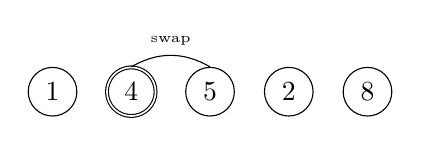
\begin{tikzpicture}
                \path (0,0) node[circle,draw] (A) {1};
                \path node[circle,draw,double,right of=A] (B) {4};
                \path node[circle,draw,right of=B] (C) {5};
                \path node[circle,draw,right of=C] (D) {2};
                \path node[circle,draw,right of=D] (E) {8};
            
                \begin{scope}[every node/.append style={midway}]
                  \draw[bend left] (B.north) edge node[above]{\tiny swap} (C.north);
                \end{scope}
              \end{tikzpicture}
        \end{subfigure}

        \rulesep

        \begin{subfigure}[b]{\textwidth}
            \centering
              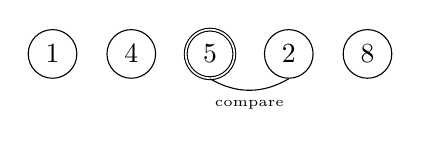
\begin{tikzpicture}
                \path (0,0) node[circle,draw] (A) {1};
                \path node[circle,draw,right of=A] (B) {4};
                \path node[circle,draw,double,right of=B] (C) {5};
                \path node[circle,draw,right of=C] (D) {2};
                \path node[circle,draw,right of=D] (E) {8};
            
                \begin{scope}[every node/.append style={midway}]
                  \draw[bend right] (C.south) edge node[below]{\tiny compare} (D.south);
                \end{scope}
              \end{tikzpicture}
        \end{subfigure}
        \begin{subfigure}[b]{\textwidth}
            \centering
              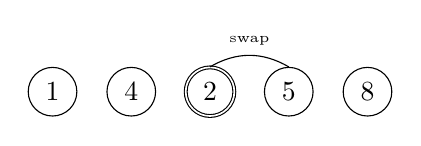
\begin{tikzpicture}
                \path (0,0) node[circle,draw] (A) {1};
                \path node[circle,draw,right of=A] (B) {4};
                \path node[circle,draw,double,right of=B] (C) {2};
                \path node[circle,draw,right of=C] (D) {5};
                \path node[circle,draw,right of=D] (E) {8};
            
                \begin{scope}[every node/.append style={midway}]
                  \draw[bend left] (C.north) edge node[above]{\tiny swap} (D.north);
                \end{scope}
              \end{tikzpicture}
        \end{subfigure}
        
        \rulesep
        
        \begin{subfigure}[b]{\textwidth}
            \centering
              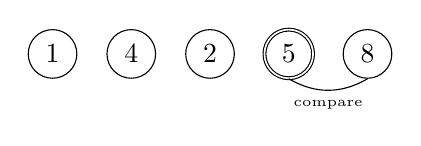
\begin{tikzpicture}
                \path (0,0) node[circle,draw] (A) {1};
                \path node[circle,draw,right of=A] (B) {4};
                \path node[circle,draw,right of=B] (C) {2};
                \path node[circle,draw,double,right of=C] (D) {5};
                \path node[circle,draw,right of=D] (E) {8};
            
                \begin{scope}[every node/.append style={midway}]
                  \draw[bend right] (D.south) edge node[below]{\tiny compare} (E.south);
                \end{scope}
              \end{tikzpicture}
        \end{subfigure}
        \begin{subfigure}[b]{\textwidth}
            \centering
              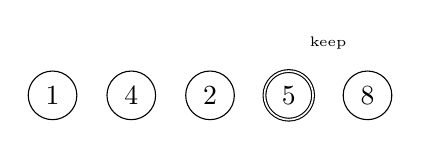
\begin{tikzpicture}
                \path (0,0) node[circle,draw] (A) {1};
                \path node[circle,draw,right of=A] (B) {4};
                \path node[circle,draw,right of=B] (C) {2};
                \path node[circle,draw,double,right of=C] (D) {5};
                \path node[circle,draw,right of=D] (E) {8};
            
                \begin{scope}[every node/.append style={midway}]
                  \draw[bend left] (D.north) edge[draw=none] node[above]{\tiny keep} (E.north);
                \end{scope}
              \end{tikzpicture}
        \end{subfigure}
        
        \rulesep
        
        \begin{subfigure}[b]{\textwidth}
            \centering
              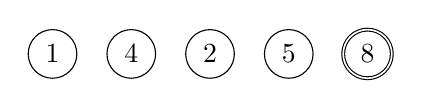
\begin{tikzpicture}
                \path (0,0) node[circle,draw] (A) {1};
                \path node[circle,draw,right of=A] (B) {4};
                \path node[circle,draw,right of=B] (C) {2};
                \path node[circle,draw,right of=C] (D) {5};
                \path node[circle,draw,double,right of=D] (E) {8};
              \end{tikzpicture}
        \end{subfigure}
        \begin{subfigure}[b]{\textwidth}
            \centering
              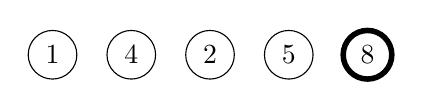
\begin{tikzpicture}
                \path (0,0) node[circle,draw] (A) {1};
                \path node[circle,draw,right of=A] (B) {4};
                \path node[circle,draw,right of=B] (C) {2};
                \path node[circle,draw,right of=C] (D) {5};
                \path node[circle,draw,line width=2pt,right of=D] (E) {8};
              \end{tikzpicture}
        \end{subfigure}
\end{figure}

At the end of the second pass we will end up with a list like this:

\begin{figure}[htp]
    \centering
    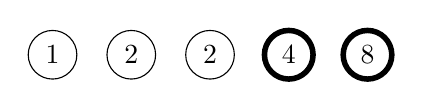
\begin{tikzpicture}
        \path (0,0) node[circle,draw] (A) {1};
        \path node[circle,draw,right of=A] (B) {2};
        \path node[circle,draw,right of=B] (C) {2};
        \path node[circle,draw,line width=2pt,right of=C] (D) {4};
        \path node[circle,draw,line width=2pt,right of=D] (E) {8};
    \end{tikzpicture}
\end{figure}

Maybe you already noticed, but this means we have to go through the whole list as many times as elements in the list, if the list has 5 elements we have to go through the list 5 times or as mathematician likes to say, we have to check $n^2$ elements, we say the efficiency of bubble sort is then $\mathcal{O}(n^2)$.

Moving this algorithm to Python this is simple, we just need to go through the list $n$ times, or well, do a loop inside another loop. Notice the usage of the typing package and a \textit{generic}, it will return a list of the same type of the entry list.

% Python code
\begin{listing}
\caption{Bubble sort in Python}
\begin{minted}{python}
def bubble_sort(elems: List[T]) -> List[T]:
    if not elems:
        return elems
    
    for mx in range(len(elems), 0, -1):
        for idx in range(1, mx):
            if elems[idx - 1] > elems[idx]:
                elems[idx - 1], elems[idx] = elems[idx], elems[idx - 1]

    return elems
\end{minted}
\end{listing}

\subsection{Selection sort}

Selection sort is another very simple sorting algorithm, the idea is simple: we pick the first element in the sequence and then \textit{search} the smaller element in the remaining pack and if found swap places. Selection sort uses \textit{linear search} (I will cover search algorithms later) to find the \textit{next smaller element} until the sequence is completely sorted, it is called \textit{selection sort} because of that, it \textit{selects} the next smaller element in a sequence, we try to simplify this in the figure \ref{figure:sorting_selection}.

\begin{figure}[htp]
    \centering
    \caption{Selection sort}
    \label{figure:sorting_selection}
    \begin{tikzpicture}
        \begin{scope}
            \path (0,0) node[circle,double,draw] (A) {5};
            \path node[circle,draw,right of=A] (B) {1};
            \path node[circle,draw,right of=B] (C) {4};
            \path node[circle,draw,right of=C] (D) {2};
            \path node[circle,draw,right of=D] (E) {8};
            
            \path node[above=1pt of B] (S) {};
            \path node[above=1pt of E] (T) {};
            
            \draw[->] (S.west) -- node[above] {\tiny search} (T.east);
        \end{scope}
        \begin{scope}[shift={($(A.south)+(0,-0.75cm)$)}]
            \path (0,0) node[circle,double,draw] (A1) {5};
            \path node[fill=red!10,circle,draw=red,right of=A1] (B1) {1};
            \path node[circle,draw,right of=B1] (C1) {4};
            \path node[circle,draw,right of=C1] (D1) {2};
            \path node[circle,draw,right of=D1] (E1) {8};
        \end{scope}
        \begin{scope}[shift={($(A1.south)+(0,-0.75cm)$)}]
            \path (0,0) node[circle,double,draw] (A2) {1};
            \path node[circle,draw,right of=A2] (B) {5};
            \path node[circle,draw,right of=B] (C) {4};
            \path node[circle,draw,right of=C] (D) {2};
            \path node[circle,draw,right of=D] (E) {8};
            
            \begin{scope}[every node/.append style={midway}]
                \draw[bend right] (A2.south) edge node[below]{\tiny swap} (B.south);
            \end{scope}
        \end{scope}
        \begin{scope}[shift={($(A2.south)+(0,-1cm)$)}]
            \path (0,0) node[circle,thick,draw] (A) {1};
            \path node[circle,draw,double,right of=A] (B) {5};
            \path node[circle,draw,right of=B] (C) {4};
            \path node[circle,draw,right of=C] (D) {2};
            \path node[circle,draw,right of=D] (E) {8};
        \end{scope}
        
    \end{tikzpicture}
\end{figure}

As we see, we have a lot less \textit{swapping} compared with bubble sort but we still have to go through all the elements in the list as many times as elements, so as with bubble sort, the efficiency of selection sort is $\mathcal{O}(n^2)$.

As usual, implementing this algorithm in Python is easy, a sample implementation can be see in source code \ref{code:selection-sort-python}.

\begin{listing}
\caption{Selection sort in Python}
\label{code:selection-sort-python}
\begin{minted}{python}
def selection_sort(elems: List[T]) -> List[T]:
    if not elems:
        return elems
    n = len(elems)
    for i in range(0, n):
        smidx = i
        for j in range(i + 1, n):
            if elems[smidx] > elems[j]:
                smidx = j
        if i != smidx:
            elems[i], elems[smidx] = elems[smidx], elems[i]
    return elems
\end{minted}
\end{listing}

Selection sort, while very similar in functionality and worst case scenario to bubble sort, is more efficient than the later because two reasons:

\begin{itemize}
    \item We do a lot less swapping compared to bubble sort, in general we will do $n$ swaps while bubble sort will need $n^2$.
    \item The number of comparisons is less, in general we see we do a simple arithmetic series with comparisons (that is $(n-1)+n(n-2)+\dots+2+1$ or $\frac{n(n-1)}{2}$ but we can simplify it to $\frac{n^2}{2}$.
\end{itemize}

\subsection{Insertion sort}

This is another simple sorting algorithm, the idea is to keep all the elements at the front of the sequence sorted, to do that we move all elements in the left to the right that are greater than the current element and then \textit{insert} the element to the correct position.

\begin{figure}[htp]
    \centering
    % First pass
    \begin{tikzpicture}
        \begin{scope}
            \path (0,0) node[circle,draw] (A) {5};
            \path node[circle,draw,right of=A] (B) {1};
            \path node[circle,draw,right of=B] (C) {4};
            \path node[circle,draw,right of=C] (D) {2};
            \path node[circle,draw,right of=D] (E) {8};
        \end{scope}
        \begin{scope}[shift={($(A.south)+(0,-1.5cm)$)}]
            \path (0,0) node[circle,thick,draw] (A1) {5};
            \path node[circle,draw,dotted,left of=A1] (space1) {};
            \path node[circle,draw,double,right of=A1] (B1) {1};
            \path node[circle,draw,right of=B1] (C1) {4};
            \path node[circle,draw,right of=C1] (D1) {2};
            \path node[circle,draw,right of=D1] (E1) {8};
            
            \path node[above=8pt of A1.west] (S) {};
            \path node[above=8pt of A1.east] (T) {};
            
            \draw[->] (S.west) -- node[above] {\tiny shift} (T.east);
            
            \begin{scope}[every node/.append style={midway}]
                \path[bend left,->] (B1.south) edge node[below]{\tiny move} (space1.south);
            \end{scope}
        \end{scope}
        
        % Second pass    
        \begin{scope}[shift={($(A1.south)+(0,-1.5cm)$)}]
            \path (0,0) node[circle,thick,draw] (A2) {1};
            \path node[draw,right of=A2,circle,dotted] (space2) {};
            \path node[circle,thick,draw,right of=space2] (B2) {5};
            \path node[circle,draw,double,right of=B2] (C2) {4};
            \path node[circle,draw,right of=C2] (D2) {2};
            \path node[circle,draw,right of=D2] (E2) {8};
            
            \path node[above=8pt of B2.west] (S) {};
            \path node[above=8pt of B2.east] (T) {};
            
            \draw[->] (S.west) -- node[above] {\tiny shift} (T.east);
            
            \begin{scope}[every node/.append style={midway}]
                \path[bend left,->] (C2.south) edge node[below]{\tiny move} (space2.south);
            \end{scope}
        \end{scope}
        
        % Third pass
        % Second pass    
        \begin{scope}[shift={($(A2.south)+(0,-1.5cm)$)}]
            \path (0,0) node[circle,thick,draw] (A3) {1};
            \path node[draw,right of=A3,circle,dotted] (space3) {};
            \path node[circle,thick,draw,right of=space3] (B3) {4};
            \path node[circle,thick,draw,right of=B3] (C3) {5};
            \path node[circle,double,draw,right of=C3] (D3) {2};
            \path node[circle,draw,right of=D3] (E3) {8};
            
            \path node[above=8pt of B3.west] (S) {};
            \path node[above=8pt of C3.east] (T) {};
            
            \draw[->] (S.west) -- node[above] {\tiny shift} (T.east);
            
            \begin{scope}[every node/.append style={midway}]
                \path[bend left,->] (D3.south) edge node[below]{\tiny move} (space3.south);
            \end{scope}
        \end{scope}
        
    \end{tikzpicture}
    \caption{Insertion sort simplified}
    \label{fig:my_label}
\end{figure}

Insertion sort sounds a little difficult to understand at the beginning but it is easy if we see the difference with selection sort, in selection sort we \textit{select} the smaller element in the pack while with insertion sort we \textit{insert} the current element in its right place in the pack.

As with bubble sort and selection sort, insertion sort worst case is $\mathcal(O){n^2}$ but if we see carefully it is superior to selection sort in a few aspects:

\begin{itemize}
    \item The number of comparisons is reduced to $\frac{n^2}{4}$
    \item The number of exchanges is reduced to $\frac{n^2}{4}$
    \item Because we need to shift and exchange only elements out of order, if the list is partially order no movement of elements is done, improving the performance.
\end{itemize}

The algorithms book talk about array inversions stating that the number of exchanges and comparisons is the number of array inversions in the array. Whatever is an inversion should be mentioned in the book somewhere.

Implementing the algorithm in Python is a little different than in other languages (and that most of the examples you see in the internet). For example, a similar code to the common example in C would be in something like listing \ref{code:insert-sort-go} in Go.

\begin{listing}
\caption{Insertion sort in Go}
\label{code:insert-sort-in-go}
\begin{minted}{go}
func insert_sort(elems []int) []int {
    if elems == nil {
        return nil
    }
    
    for current := 1; current < len(elems); current++ {
        item := elems[current]
        search_idx := current
        for ; search_idx > 0 && elems[search_idx - 1] > item; search_idx-- {
            elems[search_idx] = elems[search_idx - 1]
        }
        elems[search_idx] = item
    }
    return elems
}
\end{minted}
\end{listing}

In Python the first first \code{for} loop can be done using the common \code{range(1, len(elems))} and the second loop would be easy to do with a simple \code{while} loop instead, everything else after that is exactly the same, you can see it in listing \ref{code:insert-sort-python}.

\begin{listing}
\caption{Insertion sort in Python}
\label{code:insert-sort-python}
\begin{minted}{python}
def insert_sort(elems: List[T]) -> List[T]:
    if not elems:
        return elems
    
    for idx in range(1, len(elems)):
        search_idx = idx
        item = elems[idx]
        while search_idx > 0 and elems[search_idx - 1] > item:
            elems[search_idx] = elems[search_idx - 1]
            search_idx -= 1
        elems[search_idx] = item
    
    return elems
\end{minted}
\end{listing}



\end{document}